\documentclass[a4paper,fontsize=11pt,line_length=40zw,number_of_lines=35,baselineskip=1.7zw]{jlreq}

\usepackage[margin=20truemm]{geometry}
\usepackage{graphicx}
\usepackage{xcolor}
\usepackage[breaklinks=true, pdfborder={0 0 0}]{hyperref}
\usepackage{xurl}
\usepackage{luacode}
\usepackage[style=ieee,backend=biber]{biblatex}
\addbibresource{refs.bib}
\usepackage[fleqn,tbtags]{mathtools}
\usepackage{listings} % プログラム表示のためのパッケージ
\lstset{
  basicstyle={\ttfamily},
  identifierstyle={\small},
  commentstyle={\smallitshape},
  keywordstyle={\small\bfseries},
  ndkeywordstyle={\small},
  stringstyle={\small\ttfamily}, frame={tb},
  breaklines=true, columns=[l]{fullflexible},
  numbers=left, xrightmargin=0pt, xleftmargin=3em,
  numberstyle={\scriptsize}, stepnumber=1,
  numbersep=1em, lineskip=-0.5ex
}

\begin{document}

\title{システム名}
\author{26G1012 石井陽泰}
\date{\today}
\maketitle

\section{システムの目的と概要}
% システムが何を実現するものなのか、どう役立つのか(何を模倣した動作か等)などを説明すること．

本システムは、暗所で車両や人と障害物との距離を直感的に把握できるようにする「距離インジケータ」である。
超音波距離センサで壁との距離を計測し、その結果を NeoPixel リングの光の回転速度と色、圧電ブザーのビープ周期、LCD の表示の三つで同時に提示することで、利用者が「どれくらい近づいているか」「危険域かどうか」を一瞬で判断できるようにしている。

具体的には、既存の車庫入れ支援システムや駐車警告システム\cite{gripon2026MicrocontrollerBasedCarParking}を参考にしつつ、単なる距離バー表示ではなく「距離に応じて LED パターンの進む速さが変わる」ことに重点を置いた構成にしている。
距離変化に応じて表示テンポが変化する設計は、注意喚起を直感的に行ううえで有効であり、視覚と聴覚の両方で危険度を伝えることを狙っている\cite{toneRef,pulseInRef,hcsr04Ref}。

\url{https://www.tinkercad.com/things/7TQ30WMwQnm-26g1012/editel?sharecode=MZAnpTt5TfT3vMYNU4AxtiqTfitiM_Kg8O0pw0faDh0}

\section{システム構成}
% 構成要素のリスト(表)と回路図を表示し、参照しながら接続関係や用途を説明すること．

本システムの構成要素を表\ref{tab:components}に示す。

\begin{table}[h]
  \centering
  \caption{構成要素一覧}
  \label{tab:components}
  \begin{tabular}{lll}
    \hline
    名前     & 数量 & コンポーネント                                 \\
    \hline
    U1     & 1  & Arduino Uno R3                          \\
    U3     & 1  & PCF8574 ベース, 39 (0x27) LCD 16 x 2 (I2C) \\
    DIST1  & 1  & 超音波距離センサー(4 ピン)                         \\
    PIEZO1 & 1  & 圧電                                      \\
    RING2  & 1  & NeoPixel Ring 24                        \\
    \hline
  \end{tabular}
\end{table}

回路図は図\ref{fig:circuit}に示す。
HC-SR04 の TRIG/ECHO ピンを Arduino Uno のデジタルピン 8 番と 9 番に接続し、NeoPixel Ring は 2 番ピンのデータ線と電源・GNDで制御する。
圧電ブザーは 7 番ピンから駆動し、LCD は I2C バス（SDA/SCL）経由で Arduino に接続している。

\begin{figure}[htbp]
  \centering
  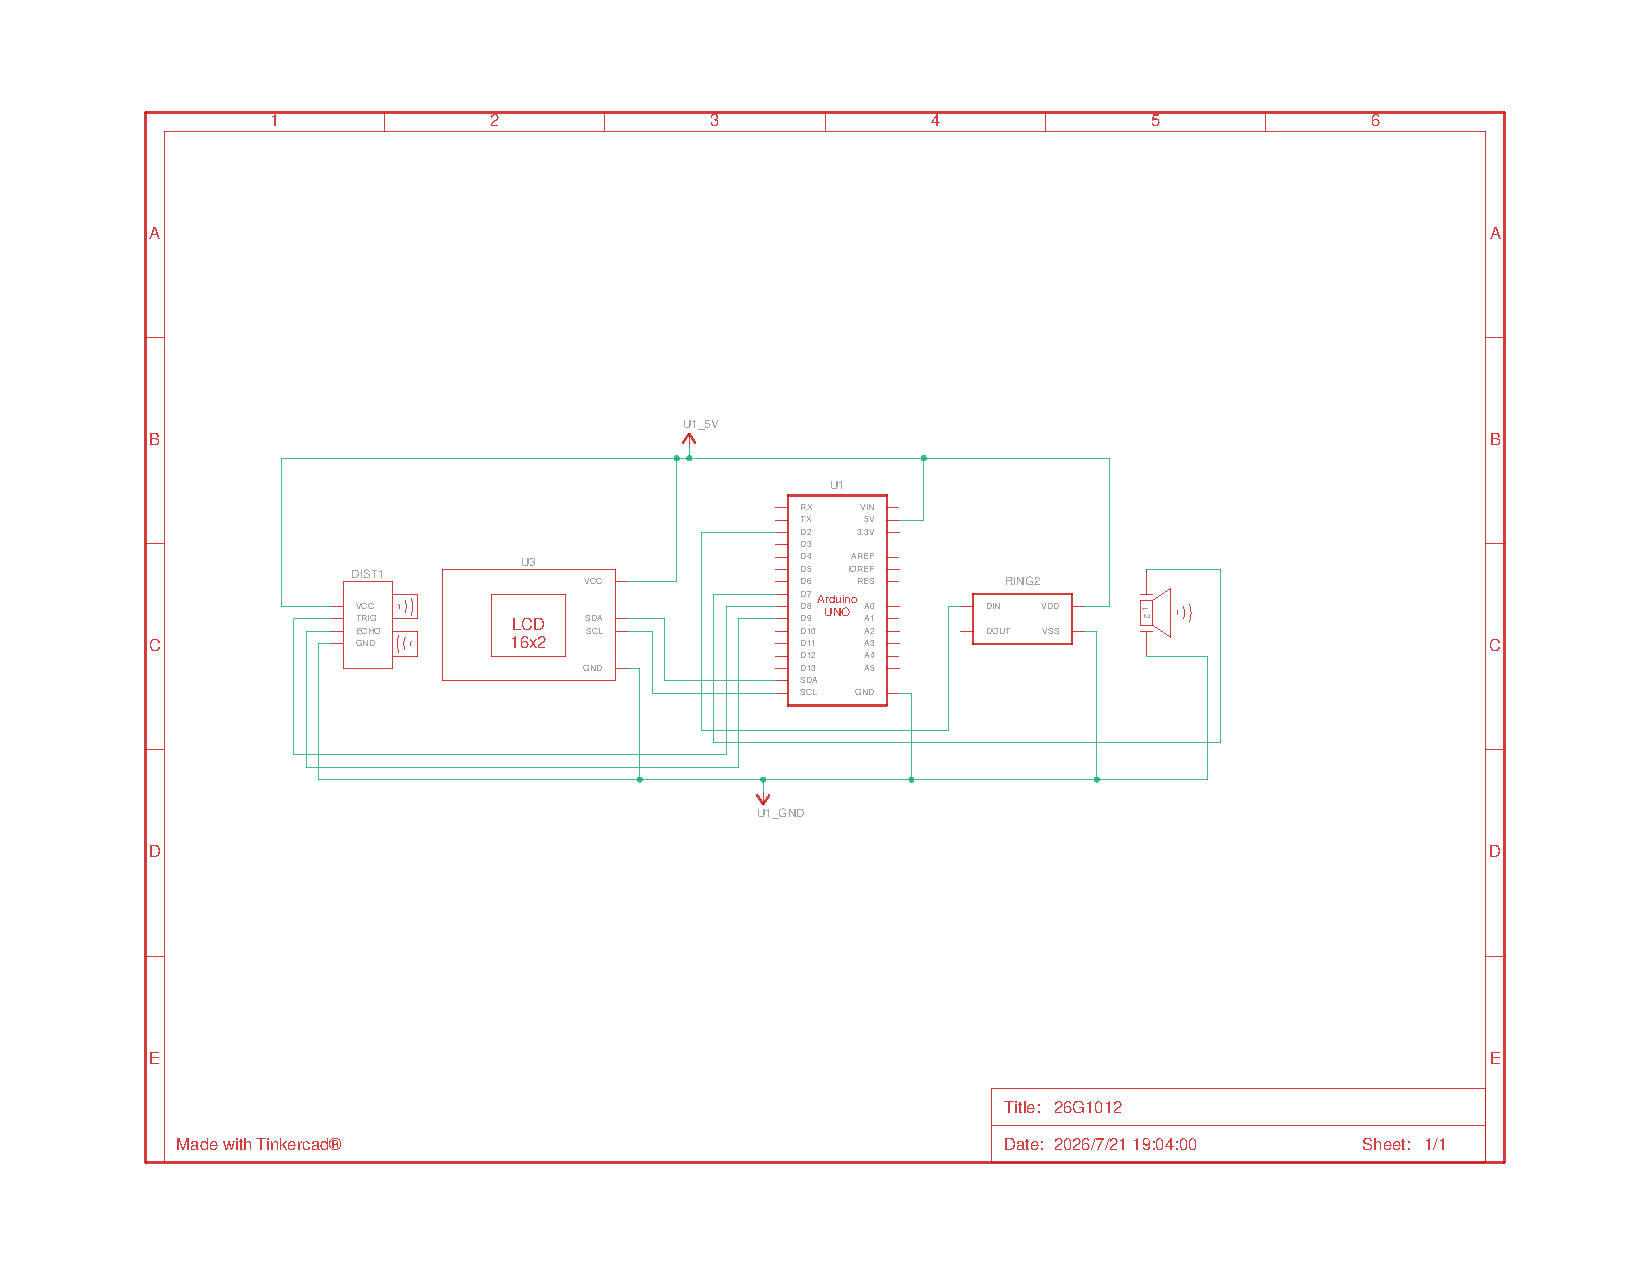
\includegraphics[width=0.92\linewidth]{Figs/seq.pdf}
  \caption{回路図}
  \label{fig:circuit}
\end{figure}

各構成要素は、次の役割に分かれる。

\begin{itemize}
  \item HC-SR04: 壁までの距離を 2〜400cm の範囲で計測する距離センサ\cite{hcsr04Ref}。
  \item Arduino Uno: センサ値を読み取り、距離に応じた状態遷移と出力制御を行う中核マイコン。
  \item NeoPixel Ring24: LED 24個をリング状に配置し、距離に応じた回転パターンと色で危険度を視覚的に表示。
  \item 圧電ブザー: 距離に応じたビープ周期で警告音を出すことで、視線が LED から外れていても危険を認識できるようにする。
  \item 16×2 I2C LCD: 距離値（cm）と SAFE / CAUTION / DANGER といった状態ラベルを文字で表示し、UI として用いる。
\end{itemize}

\section{システムの説明}
% センサがどのように物理現象を感知するのか説明すること．
% Arduinoがどのような処理を行うのか説明すること．
% 処理結果を基にアクチュエータがどう動くのか説明すること．

\subsection{超音波センサによる距離計測}

HC-SR04 超音波距離センサは、TRIG ピンに 10µs 程度の HIGH パルスを与えることで超音波を発射し、その反射波を ECHO ピンで受信する。
ECHO ピンに現れる HIGH パルスの長さは往復時間に比例し、これに音速を掛けて半分にすることで障害物までの距離を算出できる\cite{hcsr04Ref}。

本システムでは、Arduino 上で \lstinline|pulseIn(ECHO_PIN, HIGH, timeout)| を用いてパルス幅を計測し、\lstinline|duration * 0.0343 / 2.0| により距離 cm に変換している\cite{pulseInRef,hcsr04Ref}。
測定に失敗した場合には最大距離を返すことで、安全側に倒した扱いとし、誤った近距離判定で過剰に警告しないようにしている\cite{pulseInRef}。

\subsection{距離に応じた内部処理の流れ}

Arduino は、取得した距離 cm から「LED パターンの更新周期（duration）」を計算し、その周期で状態遷移ジェネレータを進める。
距離から duration へのマッピングは \lstinline|map_distance_to_duration(int distance_cm)| 関数内部で行い、近距離ほど短い duration、遠距離ほど長い duration になるように設計している。

距離と duration の関係は、以下のような二乗カーブで定義している。

\begin{itemize}
  \item \lstinline|DIST_MIN_CM|〜\lstinline|DIST_MAX_CM| を 0〜1 の区間に正規化した値を \lstinline|x| とする。
  \item \lstinline|t = x * x| とすることで、近距離側で急激に変化するカーブを作る。
  \item \lstinline|DURATION_MIN_MS|〜\lstinline|DURATION_MAX_MS| の間に \lstinline|t| をマッピングし、近距離ほど \lstinline|DURATION_MIN_MS| に近づくようにする。
\end{itemize}

これにより、距離が短くなるほど NeoPixel の回転速度とブザーのビープが一気にせわしなくなり、危険度の上昇を直感的に感じ取れるようになる。

内部状態としては、\lstinline|current_state| を 0〜23 の整数で持ち、\lstinline|STATE_COUNT = NEOPIXEL_NUM| として NeoPixel 24 個のインデックスに対応させている。
状態遷移そのものはジェネレータ関数を通して抽象化されており、距離はあくまで状態更新の速さにのみ影響し、遷移の規則そのものは距離に依存しないようにしている。

\subsection{出力の振る舞い}

計算された \lstinline|duration_ms| にしたがって、\lstinline|loop| 関数内では次の処理を行う。

\begin{itemize}
  \item 一定時間ごとに、選択されたジェネレータ（\lstinline|get_next|）を用いて \lstinline|current_state| を更新する。
  \item NeoPixel リングに対して \lstinline|render_state(current_state, distance_cm)| を呼び出し、1点ランナーとトレイルの回転パターンと距離に応じた色を表示する。
  \item 圧電ブザーには \lstinline|update_buzzer(distance_cm)| で距離に応じた状態機械を適用し、\lstinline|tone()| と \lstinline|noTone()| の切り替えで危険度に応じたリズムを表現する\cite{toneRef,noToneRef}。
  \item LCD には \lstinline|update_lcd(distance_cm)| を用いて距離値と状態ラベルを表示し、UI として扱う。
\end{itemize}

NeoPixel の色は距離レンジごとに三段階に分けており、近距離で赤、中距離で黄、遠距離で緑とすることで、色と速度の両方で危険度を多重化している。
ブザーは状態機械として実装し、\lstinline|tone()| と \lstinline|noTone()| の切り替えを明確化することで、危険度に応じたリズムを非ブロッキングに表現している\cite{toneRef,noToneRef}。

\section{プログラムの説明}

\subsection{プログラム全体の説明}

本プログラムは、超音波センサから距離を取得し、それをもとに状態遷移ジェネレータ、NeoPixel 表示、ブザー音、LCD 表示を協調制御する構造を持つ。
距離に依存するのはパターンの進む速さと色・ビープ周期であり、状態遷移のルールはジェネレータとして独立に定義されている。

中心となる考え方は、\lstinline|current_state -> next_state| を関数ポインタで表現することである。
これにより、ジェネレータを差し替えながら同じ距離 UI と同じ NeoPixel レンダリングを保ったまま、内部の遷移パターンだけをテストできるようになっている。

\subsection{関数の詳細}

\subsubsection{setup関数}

\begin{lstlisting}[firstnumber=1, caption=setup関数, label=setup]
void setup() {
  Serial.begin(9600);

  pinMode(TRIG_PIN, OUTPUT);
  pinMode(ECHO_PIN, INPUT);

  ring.begin();
  ring.setBrightness(40);
  ring.clear();
  ring.show();

  pinMode(BUZZER_PIN, OUTPUT);
  noTone(BUZZER_PIN);

  lcd.init();
  lcd.backlight();
  lcd.clear();
  lcd.setCursor(0, 0);
  lcd.print("Distance UI");

  current_state = 0;
  last_update_ms = 0;
  last_beep_ms = 0;
}
\end{lstlisting}

\begin{itemize}
  \item シリアルポートの初期化により、デバッグ用の距離値出力を可能にしている。
  \item HC-SR04 の TRIG/ECHO ピンをそれぞれ OUTPUT/INPUT に設定し、距離測定が行えるようにする。
  \item NeoPixel リングに対して begin と setBrightness を呼び、初期状態として全 LED を消灯したうえで明るさを中程度に設定する。
  \item ブザー用ピンを OUTPUT に設定し、初期状態では noTone によって無音にする。
  \item LCD を初期化し、バックライトを ON にしてからタイトル文字列 "Distance UI" を表示することで、システムが起動していることを示す。
  \item 状態変数と時間管理変数を初期化し、ループ処理が正しいタイミングからスタートするようにする。
\end{itemize}

\subsubsection{loop関数}

\begin{lstlisting}[firstnumber=1, caption=loop関数, label=loop]
void loop() {
  unsigned long now = millis();

  if (now - last_sensor_ms >= SENSOR_INTERVAL_MS) {
    last_sensor_ms = now;
    measured_distance_cm = measure_distance_cm_raw();
    filtered_distance_cm = smooth_distance_cm(filtered_distance_cm,
                                               measured_distance_cm);
  }

  int duration_ms = map_distance_to_duration(filtered_distance_cm);
  if (now - last_render_ms >= (unsigned long)duration_ms) {
    last_render_ms = now;
    current_state = get_next(current_state);
    render_state(current_state, filtered_distance_cm);
  }

  update_buzzer(filtered_distance_cm);

  if (now - last_lcd_ms >= LCD_UPDATE_INTERVAL_MS) {
    last_lcd_ms = now;
    update_lcd(filtered_distance_cm);
  }
}
\end{lstlisting}

\begin{itemize}
  \item 毎ループで現在時刻を取得し、センサ更新・LED 更新・ブザー更新・LCD 更新を個別の周期で処理する。
  \item 距離計測は一定間隔で行い、取得した値は平滑化して利用することで、表示のちらつきを抑えている。
  \item \lstinline|map_distance_to_duration(distance_cm)| により、距離を状態更新間隔に変換し、近いほど短い周期、遠いほど長い周期となるように調整する。
  \item 状態遷移は \lstinline|gens[state_logic_num]| から選ばれるジェネレータ関数ポインタを通じて実行され、\lstinline|current_state = get_next(current_state)| の形で次状態を求めている。
  \item \lstinline|render_state(current_state, distance_cm)| では、現在の状態と距離をもとに NeoPixel リングの1点ランナーとトレイルパターンを描画し、回転速度と色で危険度を視覚的に表現する。
  \item ブザーと LCD は LED 更新と独立して更新され、距離情報を音と文字でも補完している。
\end{itemize}

\subsubsection{measure\_distance\_cm関数}

\begin{lstlisting}[firstnumber=1, caption=measure\_distance\_cm関数, label=measure_distance]
int measure_distance_cm() {
  digitalWrite(TRIG_PIN, LOW);
  delayMicroseconds(2);
  digitalWrite(TRIG_PIN, HIGH);
  delayMicroseconds(10);
  digitalWrite(TRIG_PIN, LOW);

  long duration = pulseIn(ECHO_PIN, HIGH, 30000); // タイムアウト30ms
  if (duration == 0) {
    return DIST_MAX_CM; // 失敗時は「遠い」
  }
  int distance = (int)(duration * 0.034 / 2.0); // cm
  return distance;
}
\end{lstlisting}

\begin{itemize}
  \item TRIG ピンを一度 LOW にした後、10µs だけ HIGH にすることで HC-SR04 に超音波パルスの発射を指示する。
  \item ECHO ピンに現れる HIGH パルスの長さを \lstinline|pulseIn| で計測し、その値をマイクロ秒単位の往復時間とみなす。
  \item \lstinline|duration * 0.0343 / 2.0| により、音速から距離 cm を計算する。
  \item タイムアウトや異常時には \lstinline|duration == 0| となるため、その場合は \lstinline|DIST_MAX_CM| を返すことで安全側に倒した距離判定とする。
\end{itemize}

% 必要なら map_distance_to_duration, render_state, update_buzzer, update_lcd も同様に lstlisting＋説明

\section{動作例}
% スクショを使ってシステムがどのように動作するか説明すること．

ここでは、Tinkercad 上のシミュレーション画面や実機写真を用いて、距離に応じて NeoPixel リングの回転速度・色、ブザーのビープ周期、LCD の表示がどのように変化するかを示す。

\begin{itemize}
  \item 遠距離（例: 150cm 以上）では、NeoPixel の回転はゆっくりで、色は緑、ブザーは低頻度で鳴り、LCD には "SAFE" と表示される。
  \item 中距離（例: 50〜100cm）では、回転が中程度の速さになり、色は黄、ブザーのビープもやや頻繁になり、LCD には "CAUTION" と表示される。
  \item 近距離（例: 50cm 未満）では、回転がかなり速くなり、色は赤、ブザーが高頻度で鳴り、LCD には "DANGER" と表示される。
\end{itemize}

これらの動作例から、距離が変化した際に危険度がテンポと色によって視覚・聴覚的に分かることを確認できる。

\section{アピールポイント}
% 習っていないセンサを使った，センサを複数使った，制御や出力をこだわったなどを説明すること．
% 単に「２つ使いました」や「頑張りました．」のようなアピールではなく，なぜそうしたのか，その工夫によりどう良くなったのか説明すること．

本システムのアピールポイントは、以下の三点である。

\begin{itemize}
  \item 距離の UI を「数値」ではなく「パターンの進む速さ」として設計した点。単純なバー表示ではなく、距離に応じて NeoPixel の回転速度を変えることで、暗所でも危険度と距離変化の勢いを直感的に把握できるようにしている。
  \item 状態遷移ロジックを関数ポインタ（ジェネレータ）で抽象化した点。\lstinline|current_state -> next_state| を関数群として定義することで、距離 UI や表示ロジックを変えずに内部の遷移パターンだけを差し替えて比較できる。
  \item NeoPixel リング＋ブザー＋LCD という三層出力構成。視覚はリングの動きと色、聴覚はブザーのテンポ、数値は LCD の距離表示という三つのチャネルを用意することで、暗所での安全性とデバッグのしやすさの両立を図っている。
\end{itemize}

\printbibliography[title=参考文献]
\end{document}
